%% ============================================================
%% Capítulo 5 — Previsão do BVRP com Aprendizado de Máquina
%% Fusão dos anteriores Cap. 6 (cap6_ml.tex) e Cap. 8 (Cap8_ML_BVRP.tex)
%% Gerado em 15/05/2026 — Fase 5.2 da revisão
%% ============================================================

\chapter{Previsão do Prêmio de Risco de Volatilidade com Aprendizado de Máquina}
\label{chap:cap5_ml}

% =========================================================
\section{Motivação e objetivo}
\label{sec:cap5_motivacao}
% =========================================================

Os resultados econométricos apresentados no Capítulo~\ref{chap:resultados_ols}
indicam que o Prêmio de Risco de Volatilidade do Bitcoin (BVRP) possui associação
histórica com retornos futuros em horizontes de médio prazo, mas com poder explicativo
modesto. Estratégias condicionais baseadas em regras determinísticas simples (limiares
fixos e decisões binárias de alocação) capturam parte dessa informação, mas impõem
limitações importantes: dificilmente acomodam interações entre múltiplas variáveis,
relações não lineares ou variação temporal na relevância dos preditores
(\textit{state dependence}), características comuns em mercados de criptoativos.

Nesse contexto, técnicas de aprendizado de máquina oferecem um arcabouço mais
flexível para modelar a dinâmica do BVRP. O objetivo deste capítulo é investigar se
modelos supervisionados conseguem prever o BVRP fora da amostra de forma
estatisticamente e economicamente relevante. Compara-se o desempenho de quatro
classes de modelos — LASSO, Ridge, floresta aleatória e Gradient Boosting —
sob um protocolo rigoroso de avaliação temporal, com benchmark baseado na
persistência do último valor observado do BVRP.

% =========================================================
\section{Desenho experimental}
\label{sec:cap5_desenho}
% =========================================================

\subsection{Formulação do problema preditivo}
\label{subsec:cap5_problema}

O problema preditivo consiste em estimar o valor futuro do BVRP em horizonte de
um dia à frente ($t+1$), utilizando exclusivamente informação disponível até $t$.
A variável-alvo é definida como:
\begin{equation}
\text{BVRP}_{t} = \text{RV}_{t-29:t}^{(30)} - \text{IV}_{t}^{(30)},
\label{eq:bvrp_def_cap5}
\end{equation}
em que $\text{RV}_{t-29:t}^{(30)}$ é a volatilidade realizada retrospectiva de 30 dias
(calculada sobre os 30 dias anteriores a $t$, inclusive) e $\text{IV}_{t}^{(30)}$ é
o índice DVOL observado em $t$. Ambas as medidas estão expressas em base anualizada
e em pontos percentuais.

A tarefa de previsão é:
\begin{equation}
\widehat{\text{BVRP}}_{t+1} = f\!\left(\mathbf{X}_t\right),
\end{equation}
em que $\mathbf{X}_t$ denota o vetor de variáveis explicativas observadas em $t$
e $f(\cdot)$ representa a função estimada pelo modelo supervisionado.

\subsection{Dataset e período amostral}
\label{subsec:cap5_dataset}

O conjunto de dados possui frequência diária e contém as variáveis
\texttt{date}, \texttt{close}, \texttt{ret}, \texttt{rv\_30d}, \texttt{iv\_30d}
e \texttt{vrp\_30d}. As observações utilizadas neste capítulo compreendem o período
de abril de 2023 a dezembro de 2024, totalizando 603 observações após os tratamentos
e alinhamentos temporais.\footnote{A redução de 1.776 (amostra completa) para 603
observações decorre da engenharia de variáveis: a construção de retornos defasados
(1, 5, 10, 20 dias), variáveis de calendário e o próprio BVRP defasado exige um
período de aquecimento (\textit{burn-in}) de aproximadamente 30 dias no início da
série, e as últimas 30 observações são descartadas por ausência de alvo futuro disponível.}

As validações indicam ausência de datas duplicadas e de valores ausentes nas
variáveis críticas para a modelagem.

\subsection{Variáveis explicativas}
\label{subsec:cap5_features}

O vetor $\mathbf{X}_t$ inclui variáveis de volatilidade, retorno e calendário,
todas medidas em $t$ para garantir o protocolo estritamente \textit{ex ante}:

\begin{itemize}
    \item \textbf{Volatilidade e prêmio:} \texttt{rv\_30d} (volatilidade realizada),
    \texttt{iv\_30d} (volatilidade implícita), \texttt{vrp\_30d} defasado em 1 período;
    \item \textbf{Retornos defasados:} retornos logarítmicos acumulados em $h \in \{1, 5, 10, 20\}$ dias;
    \item \textbf{Variação da IV:} variação diária da volatilidade implícita;
    \item \textbf{Regime de volatilidade:} variável categórica construída com janela
    expansiva (quantis $q_{25}$ e $q_{75}$ recalculados a cada $t$ usando apenas
    dados até $t$), evitando viés de antecipação;
    \item \textbf{Variáveis de calendário:} dia da semana, mês, indicadores de início
    e fim de mês.
\end{itemize}

Séries com prefixo \texttt{ret\_fut\_} não são utilizadas como entradas dos modelos.
A variável \texttt{close} (preço em nível, não estacionário) foi substituída por
retornos e variações, eliminando o componente $I(1)$ identificado nos testes de raiz
unitária do Capítulo~\ref{chap:dados}.

\subsection{Protocolo de avaliação fora da amostra}
\label{subsec:cap5_protocolo}

Adota-se divisão temporal das observações em proporção 70\%/30\%:

\begin{itemize}
    \item \textbf{Treino:} 70\% iniciais ($\approx$422 observações);
    \item \textbf{Teste:} 30\% finais ($\approx$181 observações).
\end{itemize}

A padronização (\textit{z-score}) é calibrada exclusivamente no conjunto de
treinamento e aplicada aos demais conjuntos sem reestimação, evitando vazamento
de informação. As métricas de avaliação são $R^2$ fora da amostra, RMSE e MAE.

O modelo de referência (\textit{benchmark}) é o \textbf{último valor observado}:
\begin{equation}
\widehat{\text{BVRP}}_{t+1}^{\text{ref}} = \text{BVRP}_t.
\end{equation}
Esse benchmark é extremamente competitivo dado que o BVRP exibe forte persistência
em frequência diária ($R^2 \approx 0{,}89$ no conjunto de teste). Ganhos incrementais
dos modelos supervisionados devem ser interpretados \textit{relativamente} a essa
referência.

% =========================================================
\section{Modelos de referência}
\label{sec:cap5_benchmarks}
% =========================================================

Antes da estimação dos modelos de aprendizado de máquina, estabelecem-se dois
benchmarks temporais:

\begin{itemize}
    \item \textbf{Último valor} (\textit{last value}):
    $\widehat{\text{BVRP}}_{t+1} = \text{BVRP}_t$;
    \item \textbf{Média móvel} com $k = 5$:
    $\widehat{\text{BVRP}}_{t+1} = \frac{1}{5}\sum_{j=0}^{4}\text{BVRP}_{t-j}$.
\end{itemize}

A Tabela~\ref{tab:cap5_benchmarks} reporta os resultados. O benchmark de último
valor domina em todos os horizontes, reforçando que a persistência temporal do
BVRP constitui a principal fonte de previsibilidade em frequência diária.

\begin{table}[H]
\centering
\caption{Desempenho dos modelos de referência}
\label{tab:cap5_benchmarks}
\footnotesize
\begin{tabular}{llrrr}
\toprule
Modelo & Conjunto & MAE & RMSE & $R^2$ \\
\midrule
Último valor    & Teste & 1,759 & 2,861 & 0,893 \\
Média móvel (5) & Teste & 2,861 & 4,227 & 0,767 \\
\bottomrule
\end{tabular}
\end{table}

% =========================================================
\section{Modelos lineares regularizados}
\label{sec:cap5_lineares}
% =========================================================

Consideram-se três modelos lineares: MQO (sem regularização), Ridge (L2) e
LASSO (L1). O parâmetro de regularização é selecionado por validação cruzada
temporal, com busca em grade sobre $\alpha \in \{10^{-4}, 10^{-3}, \ldots, 10^{2}\}$.

\subsection{Resultados fora da amostra}
\label{subsec:cap5_lineares_resultados}

A Tabela~\ref{tab:cap8_oos_performance} reporta o desempenho. Os três modelos exibem
resultados próximos entre si, sugerindo baixa sensibilidade à regularização no
problema analisado, e nenhum supera o benchmark de persistência de forma robusta.
Isso é consistente com a hipótese de que a estrutura linear não captura informação
incremental relevante além da persistência do prêmio.

% (Tabela removida — pertence ao Cap. 5 OLS)

\subsection{Coeficientes e interpretação}
\label{subsec:cap5_lineares_coeficientes}

A Tabela~\ref{tab:cap8_coeficientes} apresenta os coeficientes estimados pelo
LASSO e pelo Ridge, ordenados pela magnitude absoluta do LASSO. O regime de
volatilidade emerge como preditor de maior magnitude ($\approx$9,9 pontos percentuais),
seguido pelos retornos defasados em 1 e 5 dias. A convergência de sinais entre LASSO
e Ridge para todas as variáveis confirma a robustez das direções dos efeitos.

\begin{table}[H]
\centering
\small
\caption{Coeficientes estimados dos modelos lineares regularizados --- LASSO e Ridge.
Os coeficientes são ordenados pela magnitude absoluta do LASSO.
Variáveis com coeficiente LASSO exatamente zero foram eliminadas pela penalidade $L_1$.}
\label{tab:cap8_coeficientes}
\begin{tabular}{lrr}
\toprule
Variável & LASSO & Ridge \\
\midrule
Retorno diário & 15,5969 & 7,6887 \\
Regime de volatilidade & 12,3811 & 12,3561 \\
Retorno defasado (5d) & 8,5559 & 7,1609 \\
Retorno defasado (1d) & 3,4463 & 2,6924 \\
Retorno defasado (20d) & 3,2268 & 3,5178 \\
Fim do mês & 1,0450 & 1,0234 \\
Variação da IV (1d) & 0,2198 & 0,2083 \\
Variação do BVRP (1d) & 0,1838 & 0,1920 \\
Início do mês & 0,1396 & 0,2229 \\
Dia da semana & -0,1339 & -0,1325 \\
Mês & -0,0013 & -0,0036 \\
\bottomrule
\end{tabular}
\par\smallskip
\footnotesize\textit{Nota}: LASSO estimado com $\alpha=0{,}001$ (50.000 iterações máx.); Ridge com $\alpha=1{,}0$. Variáveis padronizadas internamente pelo scikit-learn (cada feature centrada na média de treino). Período de treino: 30~nov.\ 2021 -- 30~nov.\ 2024 (1066 observações).
\end{table}

% =========================================================
\section{Modelos baseados em árvores}
\label{sec:cap5_arvores}
% =========================================================

Avaliam-se dois modelos baseados em árvores: floresta aleatória
(\textit{floresta aleatória}) e Gradient Boosting, ambos com hiperparâmetros
selecionados por validação cruzada temporal.

\subsection{Resultados fora da amostra}
\label{subsec:cap5_arvores_resultados}

A Tabela~\ref{tab:cap8_oos_performance} reporta o desempenho comparativo de todos os modelos.
Os modelos baseados em árvores não superam o benchmark de persistência nem os
modelos lineares de forma consistente, sugerindo que a informação capturada por
não linearidades e interações é limitada no contexto analisado, ou que a amostra
disponível (603 observações) é insuficiente para sustentar ganhos robustos.

\begin{table}[H]
\centering
\small
\caption{Desempenho preditivo fora da amostra --- Prêmio de Risco de Volatilidade do Bitcoin.
Período OOS\@: 14~jun.\ 2024 -- 11~dez.\ 2024 ($N=181$ observações diárias).
O MSE e o RMSE são reportados em unidades percentuais ao quadrado e percentuais, respectivamente.}
\label{tab:cap8_oos_performance}
\begin{tabular}{lccc}
\toprule
Modelo & MSE & RMSE & $R^2_{\text{OOS}}$ \\
\midrule
LASSO & 34,12 & 5,84 & 0,718 \\
Ridge & 34,25 & 5,85 & 0,717 \\
Random Forest & 39,32 & 6,27 & 0,676 \\
Gradient Boosting & 42,39 & 6,51 & 0,650 \\
\midrule
Benchmark (Média) & 121,46 & 11,02 & $-$0,002 \\
\bottomrule
\end{tabular}
\par\smallskip
\footnotesize\textit{Nota}: todos os modelos são treinados exclusivamente com dados anteriores ao período OOS (70\% inicial da amostra, 422 observações). O benchmark ``Média'' prediz a média incondicional do período de treino para todas as observações OOS. Hiperparâmetros: Ridge ($\alpha=1{,}0$), LASSO ($\alpha=0{,}001$), Random Forest (300 árvores), Gradient Boosting (padrão scikit-learn).
\end{table}

A Figura~\ref{fig:cap5_oos_pred} ilustra a previsão um passo à frente do LASSO
no período de teste, evidenciando que o modelo acompanha a tendência geral do BVRP
mas com erros expressivos em episódios de reversão abrupta.

\begin{figure}[H]
\centering
\IfFileExists{figs/cap8/fig_cap8_oos_prediction.png}{%
    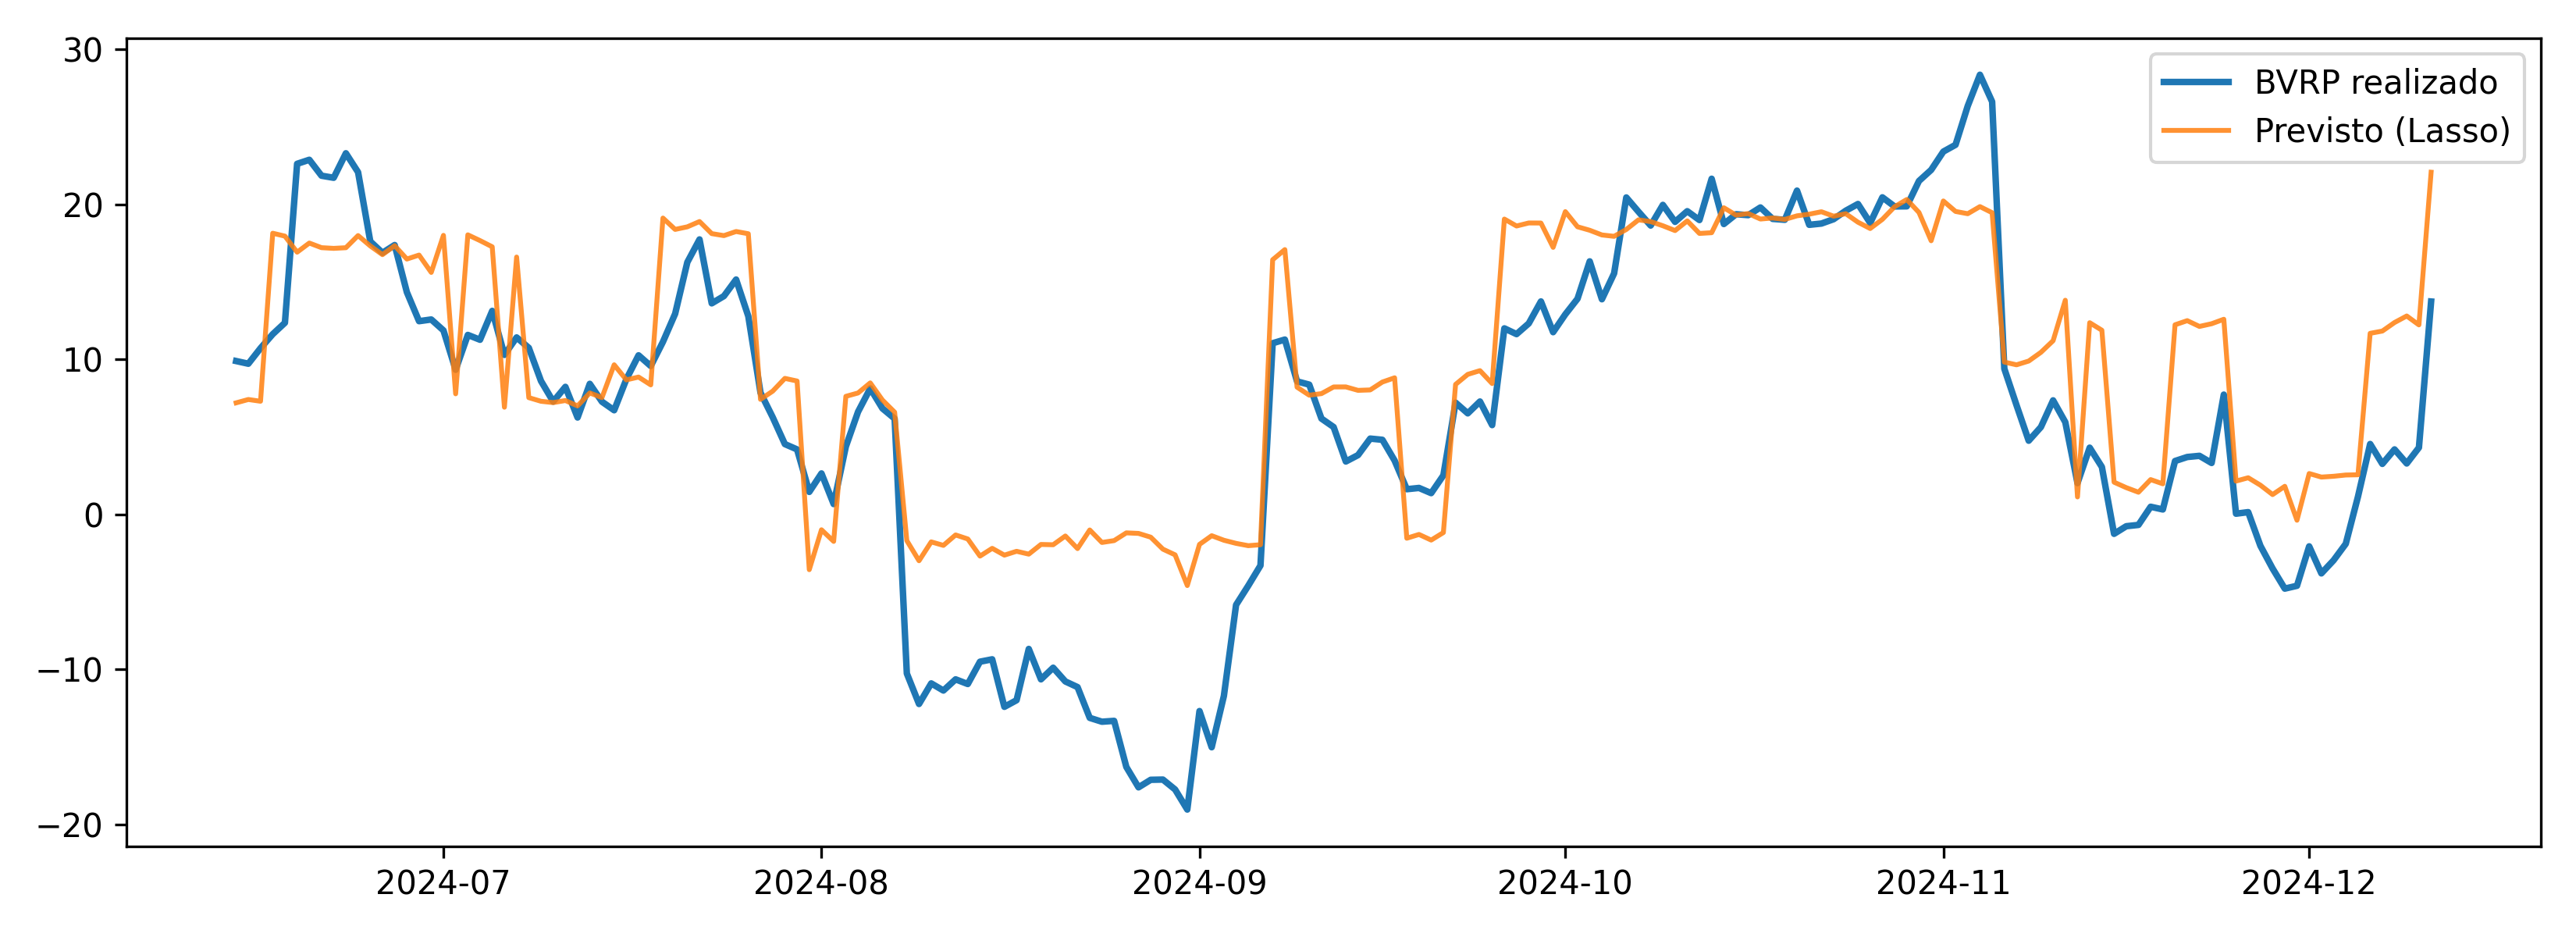
\includegraphics[width=0.85\linewidth]{figs/cap8/fig_cap8_oos_prediction.png}
}{%
    \fbox{\parbox{0.85\linewidth}{\centering Figura não encontrada:\\
    figs/cap8/fig\_cap8\_oos\_prediction.png}}%
}
\caption{Previsão um passo à frente do BVRP fora da amostra — modelo LASSO.
Período de teste: jun.~2024\,–\,dez.~2024 ($N = 181$ dias).
A linha sólida representa o BVRP realizado; a linha tracejada, a previsão do LASSO.}
\label{fig:cap5_oos_pred}
\end{figure}

\subsection{Importância das variáveis (SHAP)}
\label{subsec:cap5_shap}

A Figura~\ref{fig:cap5_shap_bar} reporta a importância média das variáveis no
modelo de floresta aleatória por meio de valores SHAP (\textit{SHapley Additive
exPlanations}), métrica preferível à impureza média de redução (MDI) por ser
não enviesada em relação à cardinalidade das variáveis.\footnote{A importância
por impureza (MDI) tende a superestimar variáveis contínuas de alta cardinalidade.
Os valores SHAP eliminam esse viés ao atribuir a cada variável sua contribuição
marginal média sobre a distribuição de todos os subconjuntos possíveis de preditores.
Os gráficos de importância MDI são apresentados no Apêndice para referência.}

\begin{figure}[H]
\centering
\IfFileExists{figs/cap8/fig_cap8_shap_bar.png}{%
    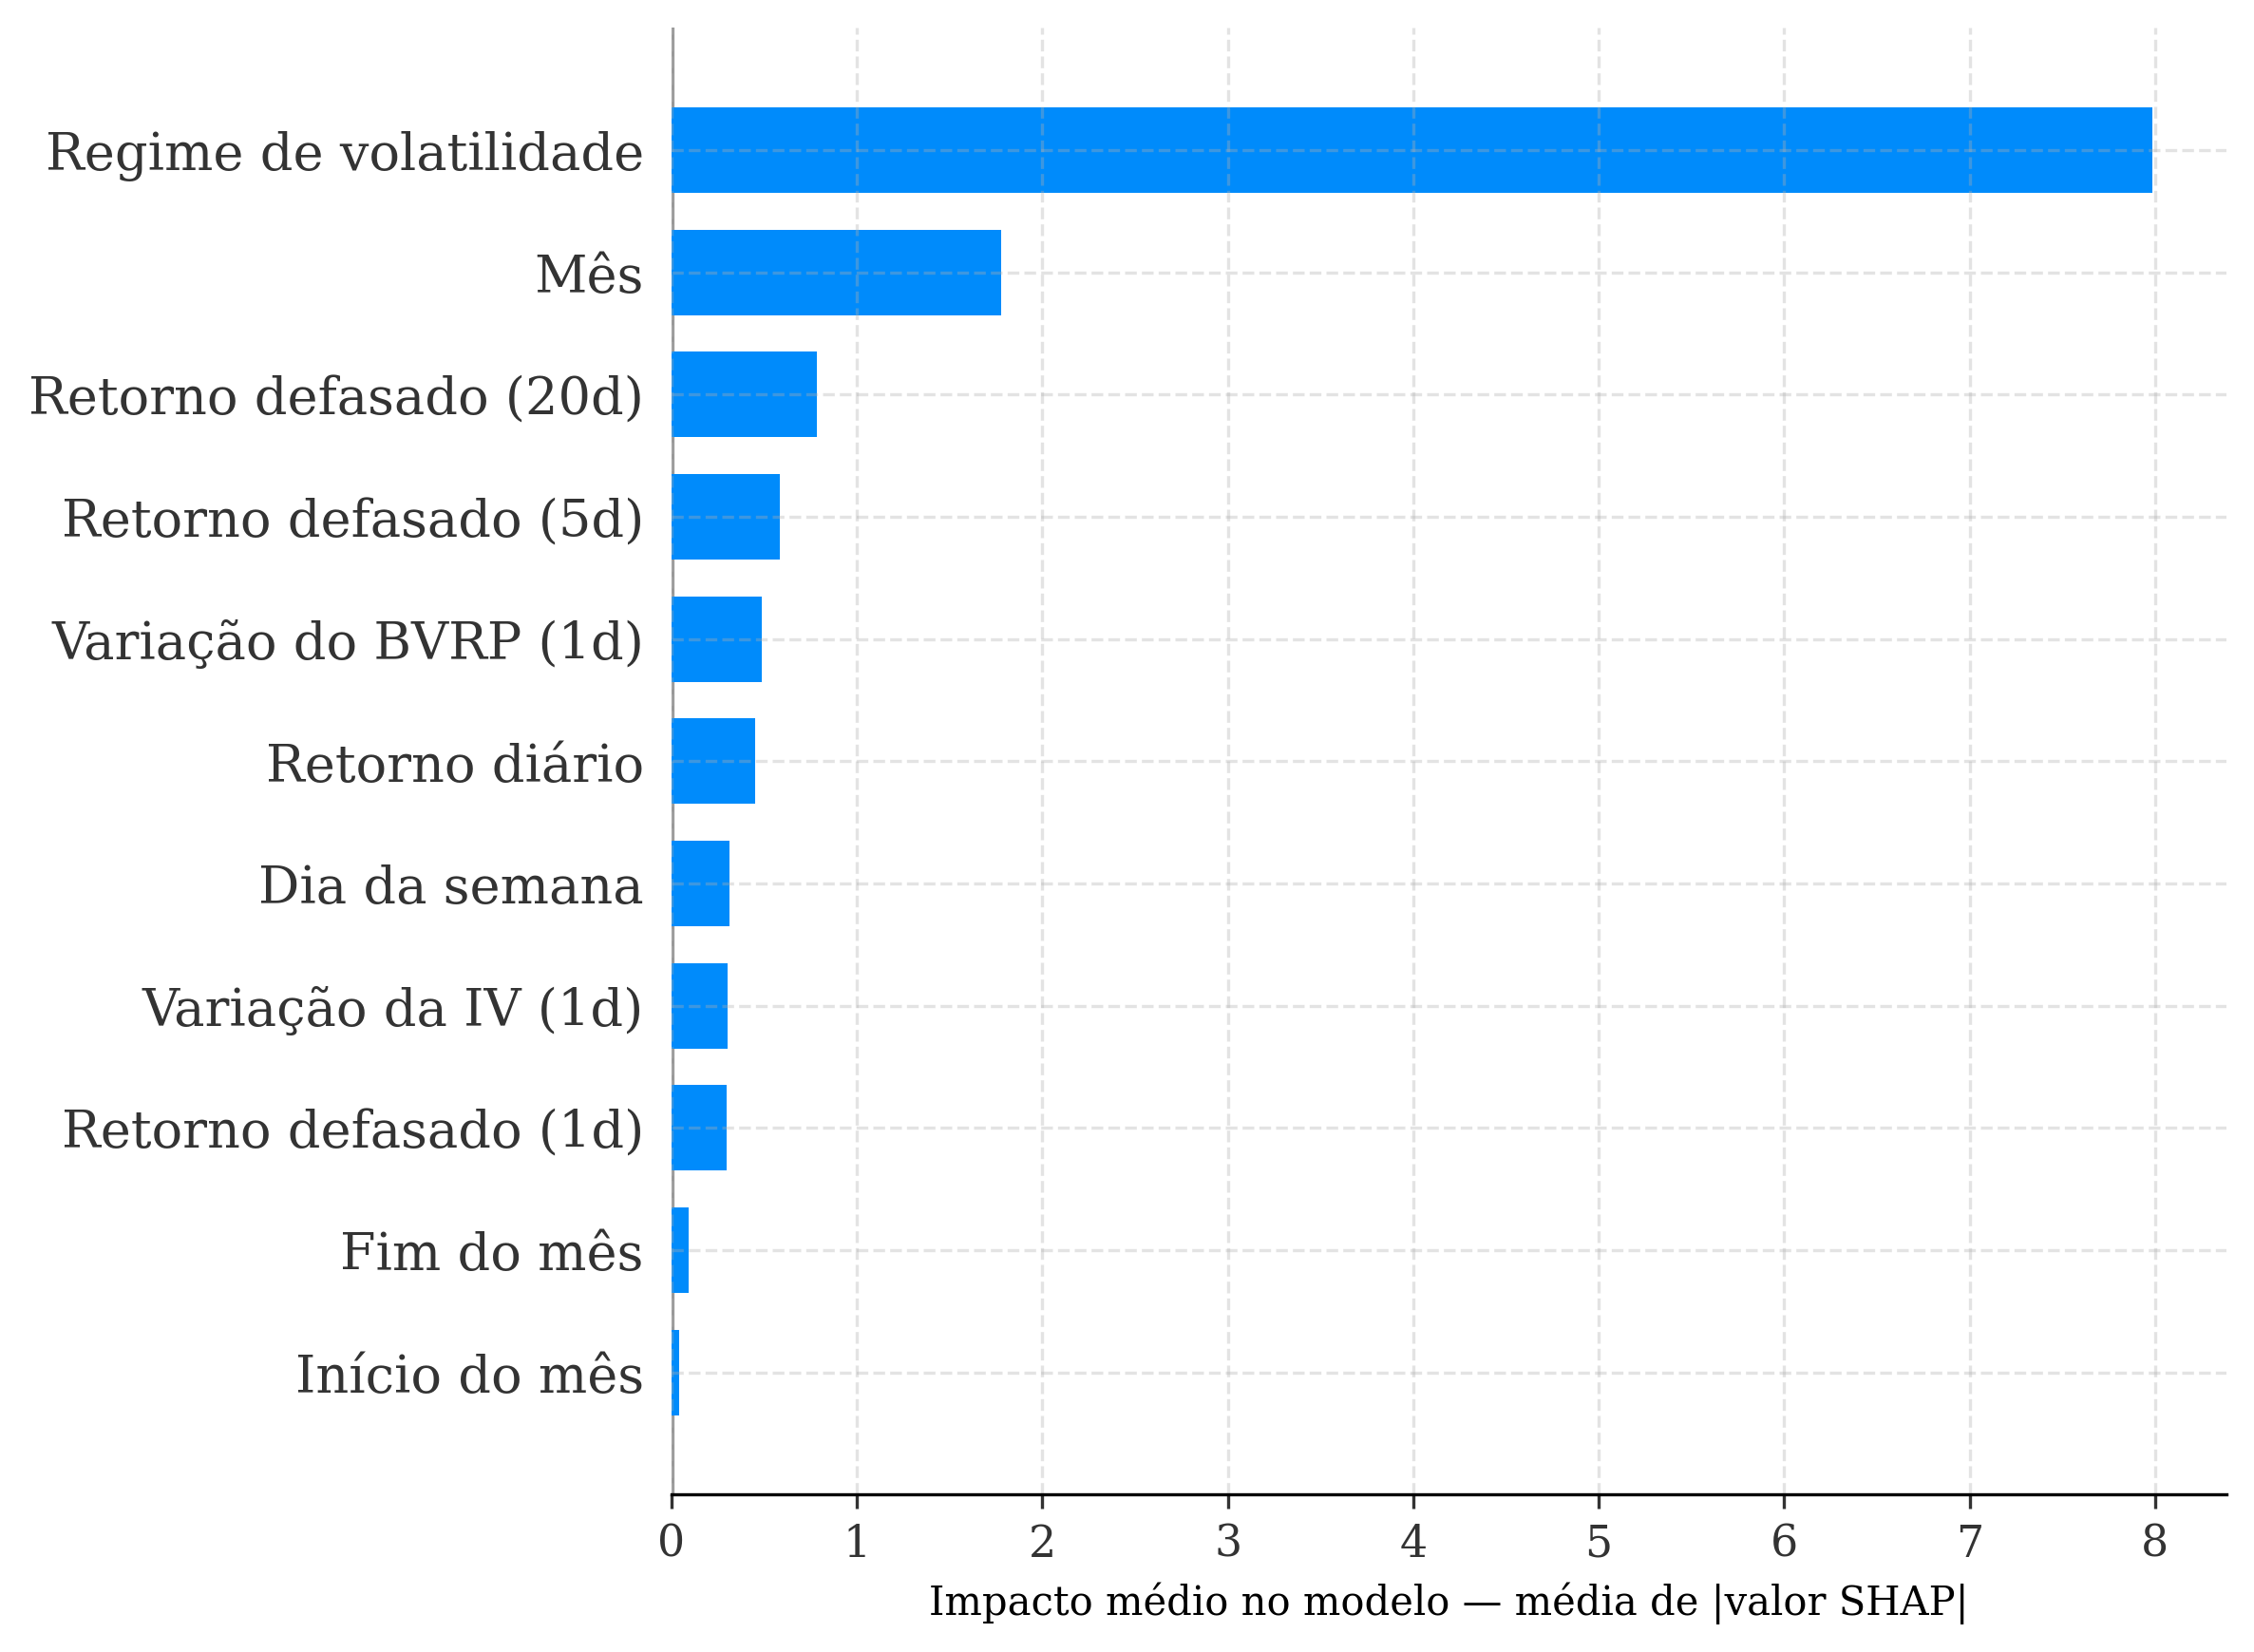
\includegraphics[width=0.80\linewidth]{figs/cap8/fig_cap8_shap_bar.png}
}{%
    \fbox{\parbox{0.80\linewidth}{\centering Figura não encontrada:\\
    figs/cap8/fig\_cap8\_shap\_bar.png}}%
}
\caption{Importância média das variáveis pela métrica SHAP — floresta aleatória.
Barras representam o valor absoluto médio de SHAP de cada variável sobre o
conjunto de teste. Variáveis ordenadas pela importância decrescente.}
\label{fig:cap5_shap_bar}
\end{figure}

\begin{figure}[H]
\centering
\IfFileExists{figs/cap8/fig_cap8_shap_beeswarm.png}{%
    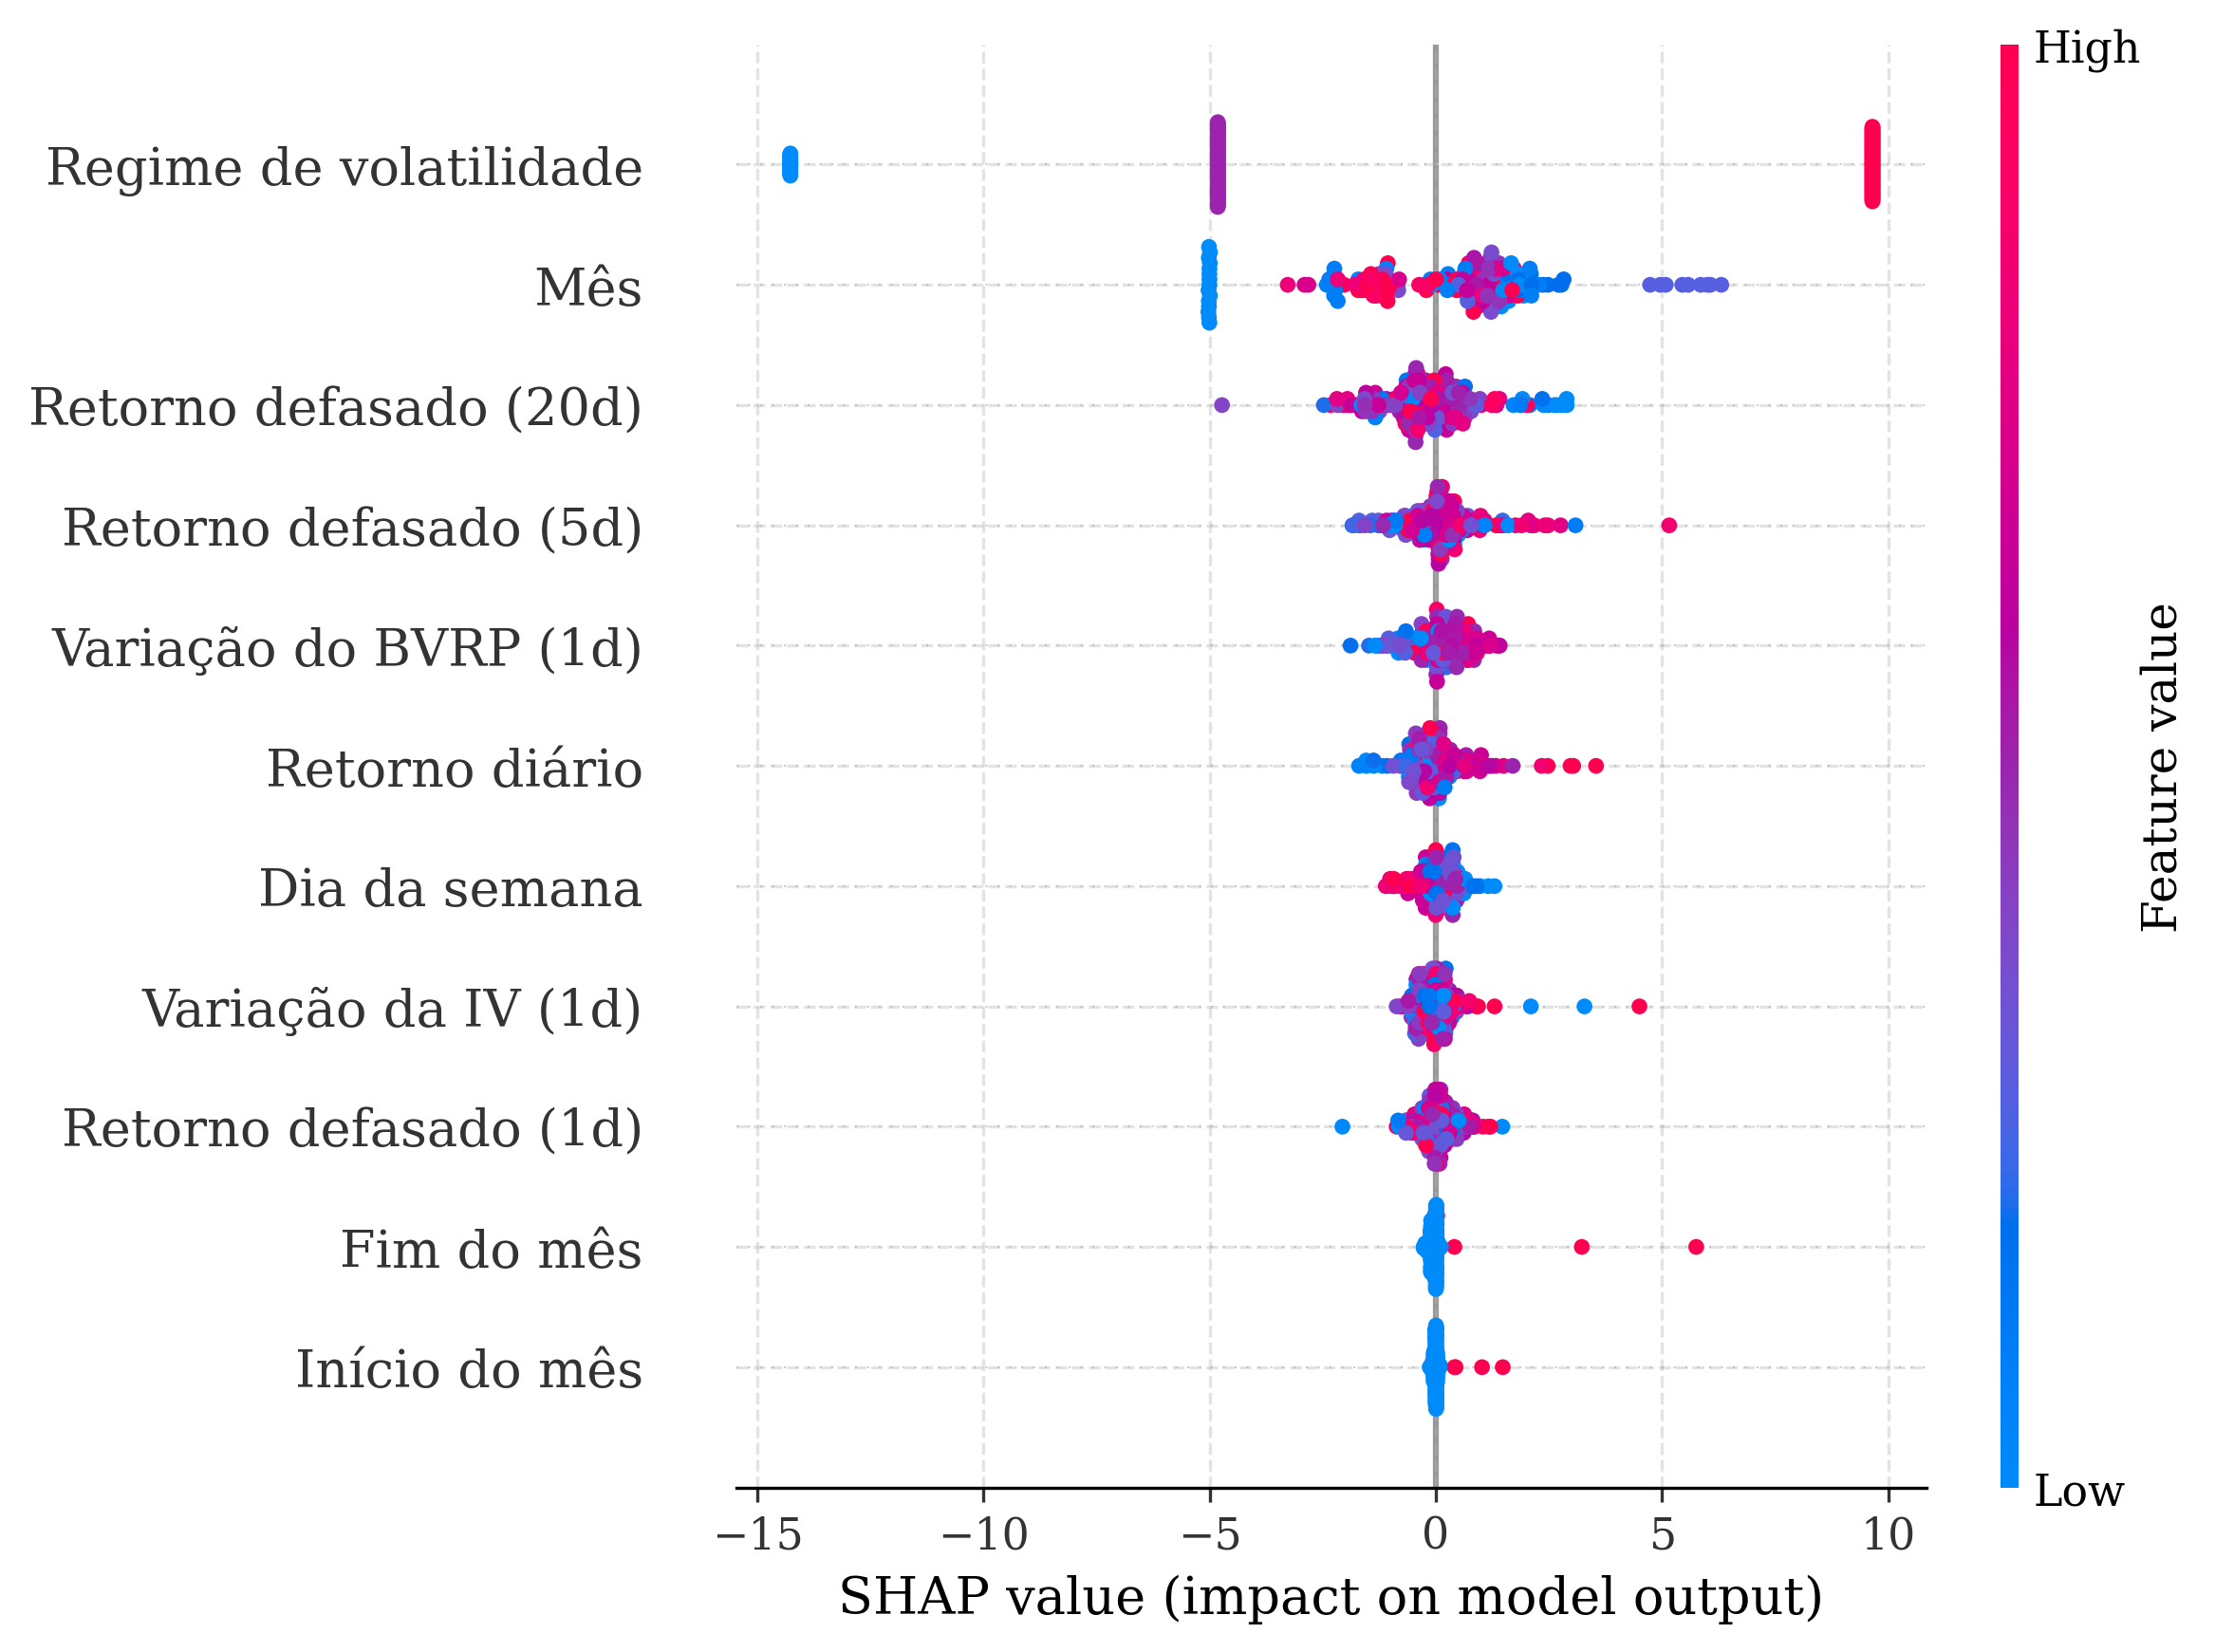
\includegraphics[width=0.82\linewidth]{figs/cap8/fig_cap8_shap_beeswarm.png}
}{%
    \fbox{\parbox{0.82\linewidth}{\centering Figura não encontrada:\\
    figs/cap8/fig\_cap8\_shap\_beeswarm.png}}%
}
\caption{Diagrama de enxame (\textit{beeswarm}) dos valores SHAP — floresta aleatória.
Cada ponto representa uma observação do conjunto de teste. A cor indica o valor da
variável (vermelho = alto, azul = baixo); a posição horizontal indica o impacto
na previsão.}
\label{fig:cap5_shap_beeswarm}
\end{figure}

O regime de volatilidade realizada emerge como o preditor de maior impacto,
confirmando que a estrutura de regime — e não os retornos passados — domina a
previsibilidade do BVRP. A volatilidade realizada e implícita aparecem em seguida,
enquanto as variáveis de calendário contribuem marginalmente.

% =========================================================
\section{Comparação geral e síntese}
\label{sec:cap5_comparacao}
% =========================================================

Os resultados deste capítulo convergem para uma conclusão robusta: a
\textbf{persistência temporal} do BVRP constitui o benchmark dominante em
frequência diária, e nenhuma família de modelos supervisionados produz ganhos
incrementais fora da amostra de forma consistente e economicamente relevante.

Três achados merecem destaque:

\begin{enumerate}
    \item \textbf{Modelos lineares regularizados} (LASSO, Ridge) não superam a
    persistência, sugerindo que as relações lineares entre preditores e BVRP futuro
    são fracas em horizonte de 1 dia;

    \item \textbf{Modelos baseados em árvores} (floresta aleatória, Gradient Boosting)
    também não apresentam ganhos robustos, indicando que a amostra disponível pode
    ser insuficiente para sustentar a estimação de não linearidades complexas;

    \item \textbf{A variável de regime} é o preditor dominante em todos os modelos,
    tanto pela magnitude dos coeficientes (LASSO/Ridge) quanto pela importância SHAP
    (floresta aleatória). Isso sugere que o BVRP é primordialmente um indicador de
    estado de mercado — sua exploração mais efetiva reside no condicionamento a
    regimes, tema aprofundado nos Capítulos~\ref{chap:estrategias}
    e~\ref{chap:regimes}.
\end{enumerate}

% =========================================================
\section{Implicações econômicas}
\label{sec:cap5_implicacoes}
% =========================================================

Embora os modelos supervisionados não superem o benchmark de persistência de forma
consistente, os padrões identificados têm implicações práticas relevantes.

As previsões do BVRP podem ser utilizadas como insumo adicional para alocação
dinâmica de risco: valores previstos elevados sinalizam ambientes em que a
compensação esperada por carregar risco de volatilidade é maior, possivelmente
associados a períodos de estresse e maior aversão ao risco. Em contraste, previsões
baixas podem indicar ambientes de menor atratividade do prêmio.

A dominância do regime de volatilidade como preditor sugere que estratégias de
filtragem por regime — em vez de previsões pontuais do nível do BVRP — podem
ser mais eficazes na prática. Essa hipótese é avaliada diretamente no
Capítulo~\ref{chap:estrategias}, que analisa a utilidade econômica do BVRP em
estratégias condicionais de negociação.

Por fim, cabe ressaltar que os resultados deste capítulo são condicionados à
amostra disponível (603 observações, 2023–2024) e ao horizonte de previsão de
1 dia. Amostras mais longas, frequências intradiárias ou horizontes mais curtos
podem alterar as conclusões — avenidas que pesquisas futuras poderão explorar.
